\chapter{Implementare, teste}

În aceast capitol vom prezenta aplicația, începând de la arhitectură, continuând apoi spre funcționalitatea oferită. Idea este să punem in aplicare conceptele teoretice de la capitolele anterioare, punând accent pe algoritmii de la secțiunea Aritmetica Eficienta, capitolul 2. Implementarea eficientă si corectă a acestor operații reprezintă un prim pas foarte important spre dezvoltarea de aplicații criptografice folosite în lumea reală, precum ECDSA.
\\ Pentru implementare am ales limbajul de programare Python, versiunea 3.5.2, iar hardware-ul folosit in tabelele de test este: Quad Core CPU, i7-4700HQ, 2.4 GHz, 64 bit OS, 16 GB RAM.

\section{Arhitectura Aplicației}
%arhitectura(Inclusiv grupul folosit, curbele eliptice Nist), diagrama UML cu clasele
Prezentare

\begin{figure}[htp]
\centering
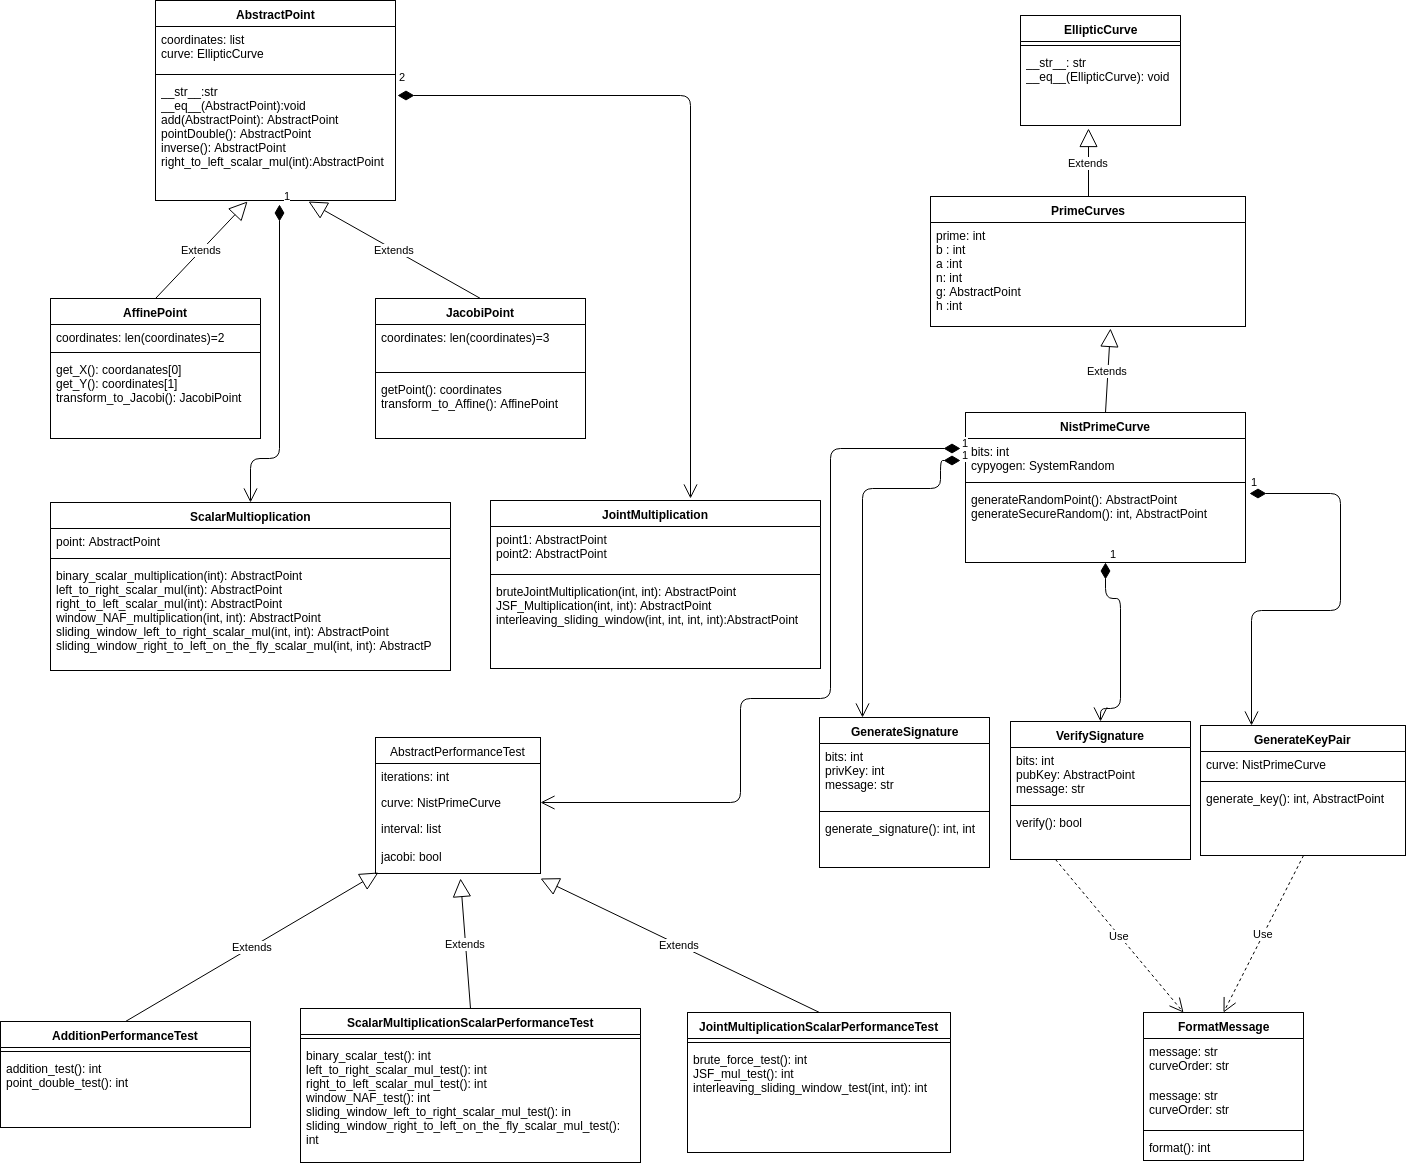
\includegraphics[width=17.5cm]{chapters/Arhitectura.png}
\caption{Arhitectura Aplicatiei}
\label{fig:lion}
\end{figure}

\section{Aritmetică}
\label{subsec:subsec02}
Prezentare

\subsection{Operația de Adunare}
In aplicatie am implementat operatia de adunare pentru coordonate Afine si pentru coordonate Jacobiene. Vom oferi formulele de calcul pentru cele tipuri de adunare si apoi vom compara eficienta celor doua implementari.

Operatiile de adunare si dublare a unui punct de pe o curba eliptica sunt operatii care au o importanta deosebita intrucat sunt folosite in fiecare algoritm de la sectiunile urmatoare(inmultire cu un scalar si inmultire multipla).
In coordonate afine algoritmul de adunare este clar, algoritmul fiind o simpla aplicare a formulelor de mai sus. Operatia cea mai costisitoare din algoritmul de mai jos e cea de invers modular(in calculul lui $\lambda$). Aceasta operatie se face cu ajutorul algoritmului lui Euclid Extins.

\begin{lstlisting} 
def add(self, other):
	if self is None:
		return other
	if other is None:
		return self

	if self == other:
		_lambda = ((3 * self.x ** 2 + self.elliptic_curve.a) 
                   * inv(2 * self.y,self.elliptic_curve.prime)) % 
                   self.elliptic_curve.prime
	else:
		_lambda = ((other.y - self.y) * 
                  inv(other.x - self.x, self.elliptic_curve.prime)) %
                  self.elliptic_curve.prime
	x3 = (_lambda ** 2 - self.x - other.x) % self.elliptic_curve.prime
	y3 = (_lambda * (self.x - x3) - self.y) % self.elliptic_curve.prime
	return Point(self.elliptic_curve, [x3, y3])
\end{lstlisting}

Ideea de la urmatorii doi algoritmi  este sa folosim un set de coordonate redundante(coordonate Jacobiene) pentru a evita calculul inversului modular.

\begin{lstlisting}
def add(self, other):
    if self is None:
        return other
    if other is None:
        return self

    u1 = (self.x * other.z ** 2) % self.curve.prime
    u2 = (other.x * self.z ** 2) % self.curve.prime
    s1 = (self.y * other.z ** 3) % self.curve.prime
    s2 = (other.y * self.z ** 3) % self.curve.prime
    if u1 == u2:
        if s1 != s2:
            return None
        else:
            return self.point_double()

    h = (u2 - u1) % self.curve.prime
    r = (s2 - s1) % self.curve.prime
    x3 = (r ** 2 - h ** 3 - 2 * u1 * h ** 2) % self.curve.prime
    y3 = (r * (u1 * h ** 2 - x3) - s1 * h ** 3) % self.curve.prime
    z3 = (h * self.z * other.z) % self.curve.prime
    return Jacobi_Point([x3, y3, z3, pow(z3, 2, self.curve.prime), 
           pow(z3, 3, self.curve.prime)], self.curve)
\end{lstlisting}

\begin{lstlisting}
def point_double(self):
    if self is None:
        return None
    if self.y == 0:
        return None
    s = (4 * self.x * self.y ** 2) % self.curve.prime
    m = (3 * self.x ** 2 + self.curve.a * self.z ** 4) % self.curve.prime
    _x = (m ** 2 - 2 * s) % self.curve.prime
    _y = (m * (s - _x) - 8 * self.y ** 4) % self.curve.prime
    _z = (2 * self.y * self.z) % self.curve.prime
    return Jacobi_Point([_x, _y, _z, pow(_z, 2, self.curve.prime), 
	   pow(_z, 3, self.curve.prime)], self.curve)
\end{lstlisting}

In continuare, vom face o comparatie intre cele doua metode de adunare, cea cu coordonate afine si cea in coordonate Jacobiene. In teste am am generat random doua numere pe o curba eliptica si le-am adunat. Am cronometrat 1000 de iteratii la fiecare test. Se poate observa per total ca adunarea in coordonate Jacobiene este de doua ori mai rapida decat cea in coordonate afine.

\subsection{Înmulțirea cu un scalar}

Putem aborda metoda problema multiplicarii cu un scalar in diferite feluri, de la cele mai ineficiente metode(apelararea functiei de adunare de cate ori este nevoie) pana la metode sofisticate si eficiente, cum ar fi inmultirea cu fereastra glisanta.

\subsubsection{Metoda Binara}

Prima metoda pe care am implementat-o este cea binara. Algoritmul consta in procesarea binara a scalarului de la cel mai nesimnificativ bit la cel mai semnificativ(de la dreapta la stanga deci). Exista si o varianta a algoritmului de la stanga la dreapta, echivalenta. Ideea este adaugam la resultat punctul P(cel care dorim sa il inmultim cu yn scalar) de fiecare data cand avem punctul P si sa dublam P-ul dupa fiecare bit parcurs.

\begin{lstlisting}
def binary_scalar_multiplication(self, d):
    P = self.point
    if d == 0:
        return None  # returnam punctul de la "infinit" daca d este 0
    if d == 1:
        return P
    result = None
    while d > 0:
        if d % 2:
            result = P.add(result)
        d //= 2
        P = P.add(P)
    return result
\end{lstlisting}

\subsubsection{Reprezentari cu semn}

Un avantaj major al curbelor eliptice, este faptul ca in grupul format de punctele de pe o astfel de curba, operatia de invers este foarte eficienta. Astfel, daca consideram 2 puncte $P, Q$ intr-un astfel de grup, putem calcula $P + Q$ si $P - Q$ cu acelasi cost computational. Aceasta observatie este foarte importanta in eficientizarea algoritmilor de inmultire cu un scalar. Calculul inversului avand un cost neglijabil din punct de vedere computational, nu este necesar sa ne limitam la $\set{0, 1}$ in reprezentarea unui scalar. Introducem astfel conceptul de reprezentare cu semn.

\begin{dfn}
[Sursa: Solinas] Fie $n\in\mathbb{N}$. O reprezentare a lui cu semn poate fi notata astfel: $n = <u_{l-1}u_{l-2}...u_1u_0>$, unde $u_i\in\set{0, -1, 1}$. Astfel $n = \sum_{i=0}^{l-1} u_i 2^{i}$. Exista o infinitate de astfel de reprezentari.
\end{dfn}
\begin{dfn}
Reprezentarea cu semn optima pentru operatia de inmultire cu un scalar este asa numita NAF, sau Non Adjacent Form. Aceasta are proprietatea ca nu exista doua elemente consecutive din reprezentarea cu semn diferite de 0.
\end{dfn}

\begin{teo}
NAF-ul are urmatoarele proprietati:
\begin{itemize}
  \item Orice numar natural are un NAF
  \item NAF-ul unui numar este unic
  \item Lungimea NAF-ului unui numar natural este cu cel mult o unitate mai mare decat expansiunea binara a numarului 
  \item NAF-ul are distanta Hamming minima dintre toate reprezentarile cu semn
\end{itemize}
\end{teo}

In continuare voi prezenta un algoritm eficient pentru calculul reprezentarii NAF.

\begin{lstlisting}
def naf(d):
    i = 0
    res = []
    while d >= 1:
        if d % 2 == 0:
            res.append(0)
        else:
            res.append(2 - d % 4)
            d -= res[i]
        d //= 2
        i += 1
    return res[::-1]
\end{lstlisting}

Avand la dispozitie metoda pentru aflarea reprezentarii cu semn a unui numar natural, putem eficientiza metoda binara. Algoritmul de la stanga la dreapta pentru calculul lui $dP$, unde d este scalarul si $P$ este un punct de pe o curba eliptica, apeleaza functia pentru reprezentare cu semn. Parcurgem aceasta reprezentare si la fiecare bit de 0 dublam rezultatul, la bitul de 1 adunam punctul $P$ sa la bitul $-1$ scadem $P$.

\begin{lstlisting}
def left_to_right_scalar_mul(self, d):
    signed_d = naf(d)
    result = None
    for i in signed_d:
        if result is None:
            result = None
        else:
            result = result.point_double()
        if i == 1:
            result = self.point.add(result)
        if i == -1:
            result = self.point.inverse().add(result)
    return result
\end{lstlisting}

Algoritmul de la dreapta la stanga functioneaza in acelasi mod, singura diferenta fiind faptul ca NAF-ul este calculat in aceasi bucla while in care calculam rezultatul final. In acea bucla descompunem scalarul, tinem bit-ul curent intr-o variabila si in functie de valoarea acestuia modificam rezultatul. 

\begin{lstlisting}
def right_to_left_scalar_mul(self, d):
    result = None
    R = self.point
    while d >= 1:
        if d % 2 == 1:
            u = 2 - (d % 4)
            d -= u
            if u == 1:
                result = R.add(result)
            else:
                result = R.inverse().add(result)
        d //= 2
        R = R.point_double()
    return result
\end{lstlisting}

\subsubsection{Metoda cu fereastra}
Algoritmii care se folososesc de reprezentarea cu semn a scalarului pot fi inbunatatiti daca avem disponibila mai multa memorie. Vom procesa $w$ cifre din scalar la o iteratie, unde $w$ reprezinta latimea ferestrei.

\begin{dfn}
Fie $w\geq 2$ un numar natural. Numim o reprezentare NAF de latime $w$ pentru un scalar $n\in\mathbb{N}$, notata cu $w-NAF$, un sir de numere $n = <u_{l-1}u_{l-2}...u_1u_0>$ astfel incat $|u_i| < 2^{w-1}$ si $n = \sum_{0}^{l-1}u_i2^i$ astfel incat cel mult una din $w$ cifre consecutive din sir este diferita de 0.
\end{dfn}

Un algoritm eficient pentru calculul $w-NAF$ va fi prezentat in continuare. Functia mods este modulo cu semn, adica pentru un scalar $d$, avem $d$ mods $2^w=u$, unde u este un numar intreg care satisface $u\equiv d$ mod $2^w$ si $-2^{w-1}\leq u\leq 2^{w-1}$.

\begin{lstlisting}
def w_NAF(d, w):
    i = 0
    res = []
    while d >= 1:
        if d % 2 == 0:
            res.append(0)
        else:
            res.append(mods(d, w))
            d -= res[i]
        d //= 2
        i += 1
    return res[::-1]
\end{lstlisting}

Metoda cu fereseatra reprezinta o generalizare a algoritmului de inmultire precedent, aducand un plus de performanta prin scaderea numarului de adunari necesare in calculul multiplului unui punct oarecare $P$ de pe o curba eliptica. Aici vom folosi $w-NAF$ in loc de $NAF$. In algoritm vom precalcula si stoca valorile pentru $iP$ si $i\in\set{1, 2^{w-1}}$. Astfel cand parcurgem $w-NAF$ -ul numarului in functie de cifra gasita vom aduna sau scadea din rezultat valoarile potrivite din multimea de valori precalculate.

\begin{lstlisting}
def window_NAF_multiplication(self, d, w):
    d = w_NAF(d, w)
    _P = {}
    for i in range(1, 2**(w-1), 2):
        _P[i] = self.right_to_left_scalar_mul(i)
    Q = None
    for i in range(0, len(d)):
        if Q is None:
            Q = None
        else:
            Q = Q.point_double()
        if d[i] != 0:
            if d[i] > 0:
                Q = _P[d[i]].add(Q)
            else:
                Q = _P[-d[i]].inverse().add(Q)
    return Q
\end{lstlisting}

\subsubsection{Metoda cu fereastra glisanta}
Pentru a eficientiza metoda cu fereastra fixa prezentata mai sus, vom procesa folosi o asa zisa "fereastra glisanta" asupra cifrelor din $w-NAF$ cu scopul de a face un compromis intre numarul de adunari si dublari. Primul algoritm apeleaza functia pt $w-NAF$ si gliseaza o fereastra de latime $w$ peste reprezentare cu semn a scalarului astfel incat valoarea in fereastra sa fie impara(pentru a reduce numarul de precalculari). Idea de la al doilea algoritm este sa calculam $w-NAF$ in aceasi bucla in care facem calculul propiu zis al multiplicarii.

\begin{lstlisting}
def sliding_window_right_to_left_scalar_mul(self, d, w):
    d = w_NAF(d, w)
    Q = None
    i = 0
    m = 2 * ((2 ** w - (-1)**w) // 3) - 1
    _P = {}
    for _i in range(1, m + 1, 2):
        _P[_i] = self.left_to_right_scalar_mul(_i)
    while i < len(d):
        if d[i] == 0:
            if Q is None:
                Q = None
            else:
                Q = Q.point_double()
            i += 1
        else:
            s = max(len(d) - i - w + 1, 0)
            s = len(d) - 1 - s
            while d[s] == 0:
                s -= 1
            u = NAF(d[i:s + 1])
            for j in range(1, i - s + 2):
                if Q is not None:
                    Q = Q.point_double()
                else:
                    Q = None
            if u > 0:
                Q = _P[u].add(Q)
            if u < 0:
                Q = Q.add(_P[-u].inverse())
            i = 1 + s
    return Q
\end{lstlisting}

\begin{lstlisting}
def sliding_window_right_to_left_on_the_fly_scalar_mul(self, k, w):
    R = self.point
    m = 2**(w-1) - 1
    Q = {}
    for i in range(1, m + 1, 2):
        Q[i] = None
    while k >= 1:
        if k % 2 == 1:
            t = mods(k, w)
            if t > 0:
                Q[t] = R.add(Q[t])
            if t < 0:
                Q[-t] = R.inverse().add(Q[-t])
            k -= t
        R = R.point_double()
        k //= 2
    for i in range(3, m + 1, 2):
        if Q[i] is not None:
            Q[1] = Q[i].right_to_left_scalar_mul(i).add(Q[1])
    return Q[1]
\end{lstlisting}

Pentru teste am decis sa aleg diferite intervale pentru marimea scalarului. Pentru fiecare test sunt rulate 1000 de iteratii cu scalari alesi random in intervalul $5-32$ biti respectiv $128-198$ si $300-384$ pentru curbele $P192$ si respectiv $P384$. Se observa eficienta metodelor cu fereastra pentru numere mari, algoritmul de inmultire care foloseste reprezentarea cu semn fiind foarte eficient pentru numere mici. De asemenea nu se observa o inbunatatirea a eficientei algoritmilor daca procesam de la stanga la dreapta sau de la dreapta la stanga sau la fereastra glisanta, cand facem calculul $w-NAF$-ului in aceasi bucla while in care calculam rezultatul.

Pentru scalari mari, cele mai bune rezultate au fost obtinute cu o fereastra glisanta de latime 4, algoritmul pierzand din eficienta pentru ferestre de latime mai mare din cauza costului mare din punct de vedere computational al precalculului. 

De asemenea putem observa beneficiul impresionant adus de folosirea coordonatelor Jacobiene, acestea aducand inbunatatiri consistente de performanta, algoritmii fiind de aproximativ cinci ori mai rapizi in aceste coordonate. 




\subsection{Inmultirea multipla}
\label{subsec:subsec04}

\begin{lstlisting}
def brute_joint_multiplication(self, k, l):
    result1 = self.point1.right_to_left_scalar_mul(k)
    result2 = self.point2.right_to_left_scalar_mul(l)
    return result1.add(result2)
\end{lstlisting}	

\begin{lstlisting}
def JSF_Multiplication(self, k, l):
    """Add using Shamir Trick, variation of algorithm 3.48, Menezez Book"""
    jsf = self.JSF(k, l)
    assert len(jsf[0]) == len(jsf[1])

    P = self.point1
    Q = self.point2

    R = None

    precom = (
              (None, Q, Q.inverse()),
              (P, P.add(Q), P.add(Q.inverse())),
              (P.inverse(), Q.add(P.inverse()), P.inverse().add(Q.inverse()))
    )

    for i, j in zip(jsf[0], jsf[1]):
        if R is None:
            R = None
        else:
            R = R.point_double()
        if i or j:
            R = precom[i][j].add(R)
        return R
\end{lstlisting}

\begin{lstlisting}
def interleaving_sliding_window(self, k, l, w1, w2):
    """Algorithm 3.5.1 menezez, 'Interleaving with NAF' """

    _P = {}
    _Q = {}
    R = None
    naf = [w_NAF(k, w1), w_NAF(l, w2)]
    _l = max([len(naf[0]), len(naf[1])])

    #precom stage
    for i in range(1, 2**(w1 - 1), 2):
        _P[i] = self.point1.right_to_left_scalar_mul(i)
    for j in range(1, 2**(w2 - 1), 2):
        _Q[j] = self.point2.right_to_left_scalar_mul(j)
 
    #padding stage
    for i in range(_l - len(naf[0])):
        naf[0].insert(i, 0)
    for i in range(_l - len(naf[1])):
        naf[1].insert(i, 0)

    for i in range(_l):
       if R is None:
            R = None
       else:
            R = R.point_double()
       for j in range(2):
            if naf[j][i] != 0:
               if naf[j][i] > 0:
                   if j == 0:
                        R = _P[naf[j][i]].add(R)
                    else:
                        R = _Q[naf[j][i]].add(R)
               else:
                    if j == 0:
                        R = _P[-naf[j][i]].inverse().add(R)
                    else:
                        R = _Q[-naf[j][i]].inverse().add(R)
    return R

\end{lstlisting}

\section{ECDSA}

\section{Eficiența implementării, Studiu Comparativ}

\begin{tabular}{ |p{3cm}||p{3cm}|p{3cm}|p{3cm}|  }
 \hline
 \multicolumn{4}{|c|}{Adunarea punctelor de pe curbe eliptice} \\
 \hline
 Curba NIST& Coordonate &Metoda &Timp de executie(secunde)\\
 \hline
 P192   & Afine    &Adunare& 5.22\\
 P192&Afine  & Dublare & 5.19\\
 P192 &Jacobiene & Adunare& 2.6\\
 P192&Jacobiene & Dublare & 2.61\\
 P224& Afine & Adunare & 6.66\\
 P224& Jacobiene & Adunare   &3.32\\
 P256& Afine  & Adunare& 8.47\\
 P256& Jacobiene  & Adunare& 4.52\\
 P384& Afine  & Adunare& 18.06\\
 P384& Jacobiene  & Adunare& 8.96\\
 \hline
\end{tabular}

\begin{tabular}{ |p{5cm}||p{3cm}|p{3cm}|p{2cm}|p{1cm}|  }
 \hline
 \multicolumn{5}{|c|}{Curba P192} \\
 \hline
 Algoritm& Coordonate &Intervalul &Fereastra &Timp\\
 \hline
 Alg Binar & Afine  &$[2^{5},2^{32}]$& - & 2.48\\
 Alg Binar&Jacobiene  & $[2^{5},2^{32}]$ & - & 0.6\\
 Alg Binar&Jacobiene  & $[2^{128},2^{192}]$ & - & 3.88\\
 Inmultire de st. la dr. & Jacobian & $[2^{5},2^{32}]$& - & 0.39\\
 Inmultire de st. la dr. & Afine & $[2^{128},2^{192}]$& - & 14.04\\
 Inmultire de st. la dr. & Jacobian & $[2^{128},2^{192}]$& - & 2.49\\
 Inmultire de dr. la st. &Afine & $[2^{128},2^{192}]$ & - & 14.33\\
 Inmultire de dr. la st. &Jacobiene & $[2^{5},2^{32}]$ & - & 0.41\\
 Inmultire de dr. la st. &Jacobiene & $[2^{128},2^{192}]$ & - & 2.52\\
 Metoda cu fereastra& Jacobiene & $[2^{5},2^{32}]$ & 3 & 0.42\\
 Metoda cu fereastra& Jacobiene & $[2^{128},2^{192}]$ & 3 & 2.38\\
 Metoda cu fereastra& Jacobiene & $[2^{128},2^{192}]$ & 4 & 2.32\\
 Fereastra glisanta st. la dr.& Jacobiene  & $[2^{5},2^{32}]$& 3 & 0.51\\
 Fereastra glisanta st. la dr.& Jacobiene  & $[2^{128},2^{192}]$& 3 & 2.68\\
  Fereastra glisanta st. la dr.& Jacobiene  & $[2^{128},2^{192}]$& 4 & 2.04\\
 Fereastra glisanta dr. la st.& Jacobiene  & $[2^{128},2^{192}]$& 3 & 2.47\\
 Fereastra glisanta dr. la st.& Jacobiene  & $[2^{128},2^{192}]$& 4 & 2.41\\
 Fereastra glisanta dr. la st.& Jacobiene  & $[2^{128},2^{192}]$& 5 & 2.58\\
 \hline
\end{tabular}

\begin{tabular}{ |p{5cm}||p{3cm}|p{3cm}|p{2cm}|p{1cm}|  }
 \hline
 \multicolumn{5}{|c|}{Curba P384} \\
 \hline
 Algoritm& Coordonate &Intervalul &Fereastra &Timp\\
 \hline
 Alg Binar & Afine  &$[2^{5},2^{32}]$& - & 5.5\\
 Alg Binar&Jacobiene  & $[2^{5},2^{32}]$ & - & 1.12\\
 Alg Binar&Jacobiene  & $[2^{300},2^{384}]$ & - & 13.98\\
 Inmultire de st. la dr. & Jacobian & $[2^{5},2^{32}]$& - & 0.66\\
 Inmultire de st. la dr. & Afine & $[2^{300},2^{384}]$& - & 59.62\\
 Inmultire de st. la dr. & Jacobian & $[2^{128},2^{192}]$& - & 8.33\\
 Inmultire de dr. la st. &Afine & $[2^{300},2^{384}]$ & - & 59.58\\
 Inmultire de dr. la st. &Jacobiene & $[2^{5},2^{32}]$ & - & 0.69\\
 Inmultire de dr. la st. &Jacobiene & $[2^{300},2^{384}]$ & - & 8.69\\
 Metoda cu fereastra& Jacobiene & $[2^{5},2^{32}]$ & 3 & 0.68\\
 Metoda cu fereastra& Jacobiene & $[2^{300},2^{384}]$ & 3 & 8.2\\
 Metoda cu fereastra& Jacobiene & $[2^{300},2^{384}]$ & 4 & 7.89\\
 Fereastra glisanta st. la dr.& Jacobiene  & $[2^{5},2^{32}]$& 3 & 0.85\\
 Fereastra glisanta st. la dr.& Jacobiene  & $[2^{300},2^{384}]$& 3 & 8.73\\
  Fereastra glisanta st. la dr.& Jacobiene  & $[2^{300},2^{384}]$& 4 & 6.46\\
 Fereastra glisanta dr. la st.& Jacobiene  & $[2^{300},2^{384}]$& 3 & 8.17\\
 Fereastra glisanta dr. la st.& Jacobiene  & $[2^{300},2^{384}]$& 4 & 7.93\\
 Fereastra glisanta dr. la st.& Jacobiene  & $[2^{300},2^{384}]$& 5 & 8.33\\
 \hline
\end{tabular}	

\begin{tabular}{ |p{5cm}||p{3cm}|p{3cm}|p{2cm}|p{1cm}|  }
 \hline
 \multicolumn{5}{|c|}{Curba P192} \\
 \hline
  Algoritm& Coordonate &Intervalul &Ferestre &Timp\\
 \hline
 Alg Brut & Afine  &$[2^{5},2^{32}]$& - & 4.85\\
 Alg Brut & Afine  &$[2^{128},2^{198}]$& - & 26.18 \\
 Alg Brut & Jacobiene  &$[2^{5},2^{32}]$& - & 1.04 \\
 Alg Brut & Jacobiene  &$[2^{128},2^{198}]$& - & 4.89 \\
 Inmultire cu JSF & Afine  &$[2^{5},2^{32}]$& - & 2.72 \\
 Inmultire cu JSF & Jacobiene  &$[2^{5},2^{32}]$& - & 0.56 \\
 Inmultire cu JSF & Jacobiene  &$[2^{128},2^{198}]$& - & 2.35 \\
 Interleaving & Jacobiene  &$[2^{5},2^{32}]$& 3, 4 & 0.66 \\
 Interleaving & Jacobiene  &$[2^{128},2^{198}]$& 3, 3 & 3.39\\
 Interleaving & Jacobiene  &$[2^{128},2^{198}]$& 3, 4 &  3.29\\
 Interleaving & Jacobiene  &$[2^{128},2^{198}]$& 4, 4 & 3.15 \\
 Interleaving & Jacobiene  &$[2^{128},2^{198}]$& 4, 5 & 3.4 \\
 Interleaving & Jacobiene  &$[2^{128},2^{198}]$& 5, 5 & 3.55 \\
 \hline
\end{tabular}

\begin{tabular}{ |p{5cm}||p{3cm}|p{3cm}|p{2cm}|p{1cm}|  }
 \hline
 \multicolumn{5}{|c|}{Curba P384} \\
  \hline
  Algoritm& Coordonate &Intervalul &Ferestre &Timp\\
 \hline
 Alg Brut & Afine  &$[2^{5},2^{32}]$& - & 10.81\\
 Alg Brut & Afine  &$[2^{128},2^{198}]$& - & 54.17 \\
 Alg Brut & Jacobiene  &$[2^{5},2^{32}]$& - & 1.69 \\
 Alg Brut & Jacobiene  &$[2^{128},2^{198}]$& - & 8.25 \\
 Inmultire cu JSF & Afine  &$[2^{5},2^{32}]$& - & 5.92 \\
 Inmultire cu JSF & Jacobiene  &$[2^{5},2^{32}]$& - & 0.9 \\
 Inmultire cu JSF & Jacobiene  &$[2^{128},2^{198}]$& - & 3.84\\
 Interleaving & Jacobiene  &$[2^{5},2^{32}]$& 3, 4 & 1.09 \\
 Interleaving & Jacobiene  &$[2^{128},2^{198}]$& 3, 3 & 5.31 \\
 Interleaving & Jacobiene  &$[2^{128},2^{198}]$& 3, 4 & 5.41 \\
 Interleaving & Jacobiene  &$[2^{128},2^{198}]$& 4, 4 & 5.23 \\
 Interleaving & Jacobiene  &$[2^{128},2^{198}]$& 4, 5 & 5.61 \\
 Interleaving & Jacobiene  &$[2^{128},2^{198}]$& 5, 5 & 5.83	 \\
 \hline
\end{tabular}

\section{Testare}
Unit teste, sper sa am timp.. 